\documentclass[a4paper,12pt]{article}

\usepackage[utf8x]{inputenc}
\usepackage[T2A]{fontenc}
\usepackage[english, russian]{babel}

% Опционно, требует  apt-get install scalable-cyrfonts.*
% и удаления одной строчки в cyrtimes.sty
% Сточку не удалять!
% \usepackage{cyrtimes}

% Картнки и tikz
\usepackage{graphicx}
\usepackage{tikz}
\usetikzlibrary{snakes,arrows,shapes}


% Некоторая русификация.
\usepackage{misccorr}
\usepackage{indentfirst}
\renewcommand{\labelitemi}{\normalfont\bfseries{--}}

% Увы, поля придётся уменьшить из-за листингов.
\topmargin -1cm
\oddsidemargin -0.5cm
\evensidemargin -0.5cm
\textwidth 17cm
\textheight 24cm

\sloppy

% Оглавление в PDF
\usepackage[
bookmarks=true,
colorlinks=true, linkcolor=black, anchorcolor=black, citecolor=black, menucolor=black,filecolor=black, urlcolor=black,
unicode=true
]{hyperref}

% Для исходного кода в тексте
\newcommand{\Code}[1]{\textbf{#1}}

\usepackage{verbatim}
\usepackage{fancyvrb}
\fvset{frame=leftline, fontsize=\small, framerule=0.4mm, rulecolor=\color{darkgray}, commandchars=\\\{\}}
\renewcommand{\theFancyVerbLine}{\small\arabic{FancyVerbLine}}



\title{Отчёт по лабораторной работе \\ <<Динамическая IP-маршрутизация>>}
\author{Руднев Дмитрий Николаевич}

\begin{document}

\maketitle

\tableofcontents

\section{Настройка сети}

\subsection{Топология сети}

Топология сети и используемые IP-адреса показаны на рисунке~\ref{fig:network}.

\begin{figure}
\centering
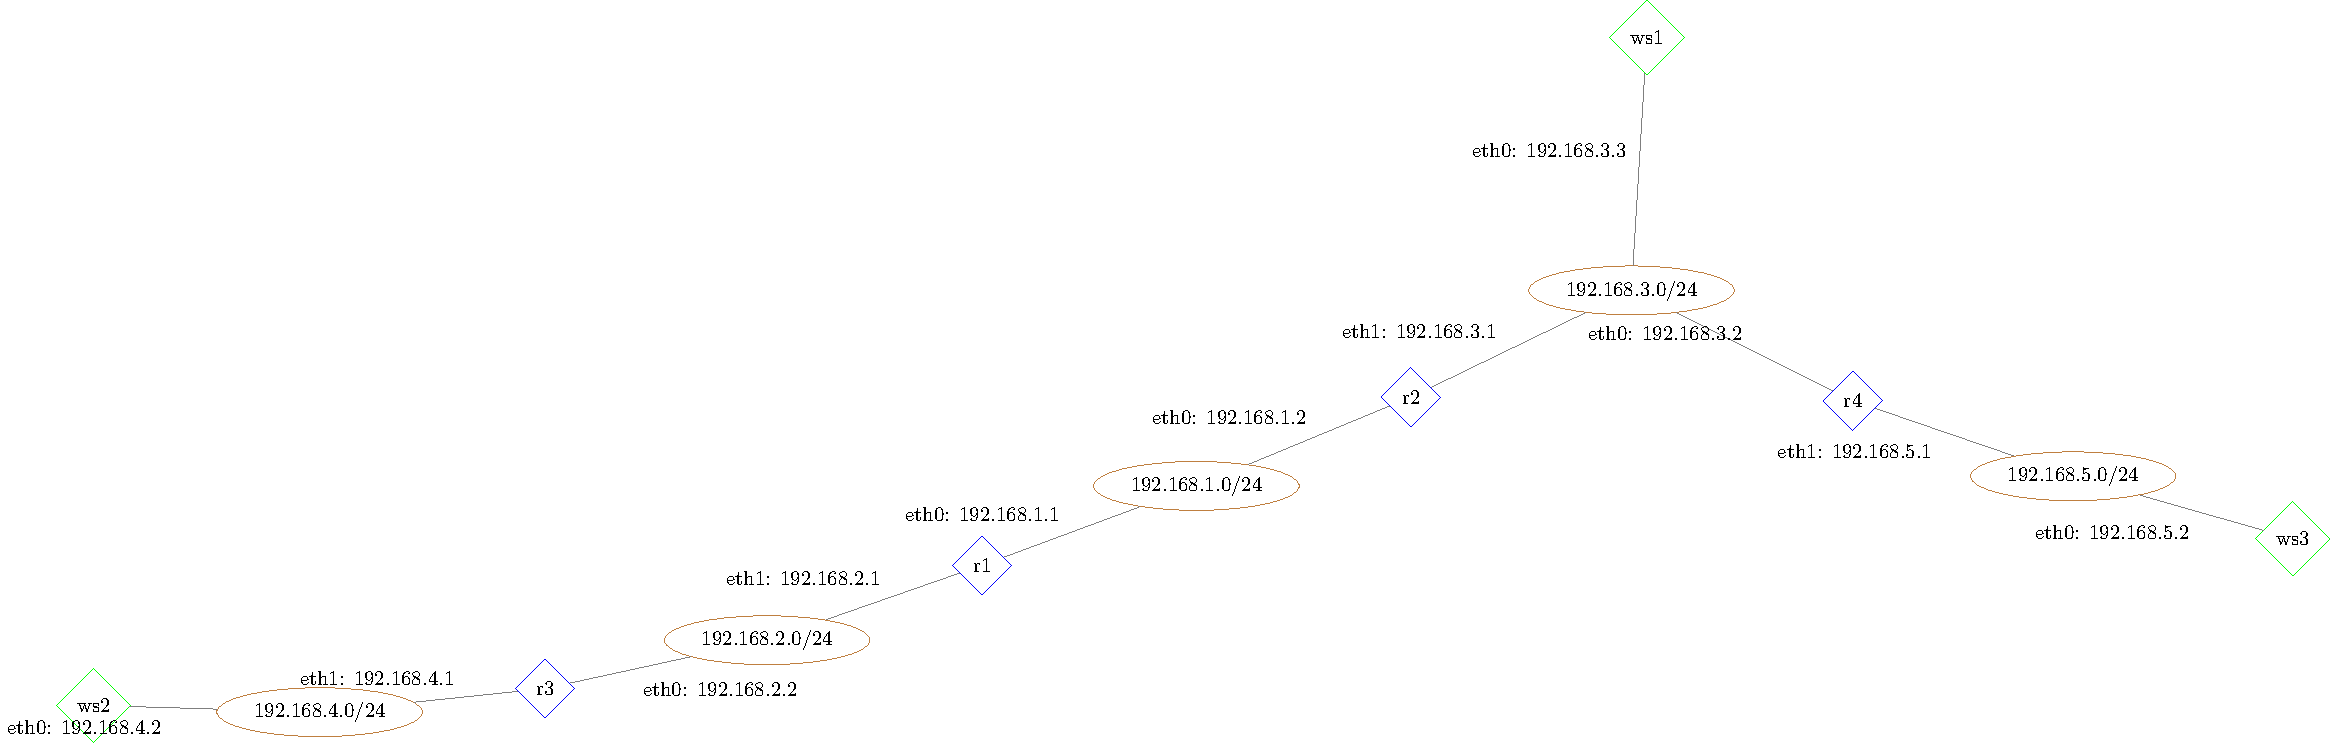
\includegraphics[width=0.8\textwidth]{includes/network_gv.pdf}
\caption{Топология сети}
\label{fig:network}
\end{figure}

Перечень узлов, на которых используется динамическая IP-маршрутизация: r1, r2, r3, r4, r5


\subsection{Назначение IP-адресов}

Ниже приведён файл сетевой настройки  маршрутизатора r1.

\begin{Verbatim}
auto lo
iface lo inet loopback

auto eth0
iface eth0 inet static
address 10.0.20.1
netmask 255.255.255.0

auto eth1
iface eth1 inet static
address 10.0.10.1
netmask 255.255.255.0
\end{Verbatim}

Ниже приведён файл сетевой настройки рабочей станции wsp1.

\begin{Verbatim}
auto lo
iface lo inet loopback

auto eth0
iface eth0 inet static
address 10.0.10.3
netmask 255.255.255.0
gateway 10.0.10.1
\end{Verbatim}



\subsection{Настройка протокола RIP}

Ниже приведен файл \Code{/etc/quagga/ripd.conf} маршрутизатора r1.

\begin{Verbatim}
! Этот настройки, касающиеся протокола RIP.
router rip

! Раскомментируйте ниже все интерфейсы, подключённые
! к сетям с другими маршрутизаторами.
network eth0
network eth1
! network eth2

! Уменьшаем значения всех таймеров для ускорения опытов.
! Рассылка: 10 сек., устаревание: 60 cек., сборка мусора: 120 сек.
timers basic 10 60 120

! Следующие две строчки заставляют маршрутизатор
! добавлять в сообщения протокола RIP все известные ему маршруты.
redistribute kernel
!redistribute connected

! Это имя файла журнала службы RIP.
! Его содержимое можно изучить в случае неполадок
log file /var/log/quagga/ripd.log
\end{Verbatim}



Ниже приведен файл \Code{/etc/quagga/ripd.conf} рабочий станции wsp1, связанной с несколькими маршрутизаторами (указать, какой).

\begin{Verbatim}
! Этот настройки, касающиеся протокола RIP.
router rip

! Раскомментируйте ниже все интерфейсы, подключённые
! к сетям с другими маршрутизаторами.
network eth0
! network eth1
! network eth2

! Уменьшаем значения всех таймеров для ускорения опытов.
! Рассылка: 10 сек., устаревание: 60 cек., сборка мусора: 120 сек.
timers basic 10 60 120

! Следующие две строчки заставляют маршрутизатор
! добавлять в сообщения протокола RIP все известные ему маршруты.
redistribute kernel
redistribute connected

! Это имя файла журнала службы RIP.
! Его содержимое можно изучить в случае неполадок
log file /var/log/quagga/ripd.log
\end{Verbatim}


\section{Проверка настройки протокола RIP}

Вывод \textbf{traceroute} от узла r4 до wsp1 при нормальной работе сети.

\begin{Verbatim}
r4:~# traceroute 10.0.10.3
traceroute to 10.0.10.3 (10.0.10.3), 64 hops max, 40 byte packets
 1  10.0.30.1 (10.0.30.1)  8 ms  0 ms  0 ms
 2  10.0.10.3 (10.0.10.3)  31 ms  1 ms  1 ms
\end{Verbatim}

Вывод \textbf{traceroute} от узла такого-т до внешнего IP (195.19.38.2 сгодится).

\begin{Verbatim}
Сюда нужно поместить вывод traceroute.
\end{Verbatim}

Вывод сообщения RIP.

\begin{Verbatim}
IP (tos 0x0, ttl 1, id 0, offset 0, flags [DF], proto UDP (17), length 112) 10.0.40.2.520 > 224.0.0.9.520: 
	RIPv2, Response, length: 84, routes: 4
	  AFI: IPv4:         0.0.0.0/0 , tag 0x0000, metric: 1, next-hop: self
	  AFI: IPv4:       10.0.10.0/24, tag 0x0000, metric: 2, next-hop: self
	  AFI: IPv4:       10.0.30.0/24, tag 0x0000, metric: 1, next-hop: self
	  AFI: IPv4:     192.168.1.0/24, tag 0x0000, metric: 1, next-hop: self
IP (tos 0x0, ttl 1, id 0, offset 0, flags [DF], proto UDP (17), length 72) 10.0.40.1.520 > 224.0.0.9.520: 
	RIPv2, Response, length: 44, routes: 2
	  AFI: IPv4:       10.0.10.0/24, tag 0x0000, metric: 2, next-hop: self
	  AFI: IPv4:       10.0.20.0/24, tag 0x0000, metric: 1, next-hop: self
\end{Verbatim}

Вывод таблицы RIP.

\begin{Verbatim}
Codes: R - RIP, C - connected, S - Static, O - OSPF, B - BGP
Sub-codes:
      (n) - normal, (s) - static, (d) - default, (r) - redistribute,
      (i) - interface

     Network            Next Hop         Metric From            Tag Time
K(r) 0.0.0.0/0          192.168.1.1           1 self              0
R(n) 10.0.10.0/24       10.0.30.1             2 10.0.30.1         0 00:51
R(n) 10.0.20.0/24       10.0.40.1             2 10.0.40.1         0 00:59
C(i) 10.0.30.0/24       0.0.0.0               1 self              0
C(i) 10.0.40.0/24       0.0.0.0               1 self              0
C(r) 192.168.1.0/24     0.0.0.0               1 self (connected:1)  0
\end{Verbatim}

Вывод таблицы маршрутизации.

\begin{Verbatim}
Таблица маршрутизации
10.0.20.0/24 via 10.0.40.1 dev eth0  proto zebra  metric 2 
192.168.1.0/24 dev eth2  proto kernel  scope link  src 192.168.1.20 
10.0.30.0/24 dev eth1  proto kernel  scope link  src 10.0.30.2 
10.0.40.0/24 dev eth0  proto kernel  scope link  src 10.0.40.2 
10.0.10.0/24 via 10.0.30.1 dev eth1  proto zebra  metric 2 
default via 192.168.1.1 dev eth2 
\end{Verbatim}

\section{Расщепленный горизонт и испорченные обратные обновления}

Поместить сюда вывод сообщения одного и того же маршрутизатор с включенным расщ. горизонтом, с включенными испорченными обновлениями, с отключённым расщ. гор.

Enabled split horizon
IP (tos 0x0, ttl 1, id 0, offset 0, flags [DF], proto UDP (17), length 112) 10.0.40.2.520 > 224.0.0.9.520: 
        RIPv2, Response, length: 84, routes: 4
          AFI: IPv4:         0.0.0.0/0 , tag 0x0000, metric: 1, next-hop: self
          AFI: IPv4:       10.0.10.0/24, tag 0x0000, metric: 2, next-hop: self
          AFI: IPv4:       10.0.30.0/24, tag 0x0000, metric: 1, next-hop: self
          AFI: IPv4:     192.168.1.0/24, tag 0x0000, metric: 1, next-hop: self

Disabled split horizon
IP (tos 0x0, ttl 1, id 0, offset 0, flags [DF], proto UDP (17), length 152) 10.0.40.2.520 > 224.0.0.9.520: 
	RIPv2, Response, length: 124, routes: 6
	  AFI: IPv4:         0.0.0.0/0 , tag 0x0000, metric: 1, next-hop: self
	  AFI: IPv4:       10.0.10.0/24, tag 0x0000, metric: 2, next-hop: self
	  AFI: IPv4:       10.0.20.0/24, tag 0x0000, metric: 2, next-hop: 10.0.40.1
	  AFI: IPv4:       10.0.30.0/24, tag 0x0000, metric: 1, next-hop: self
	  AFI: IPv4:       10.0.40.0/24, tag 0x0000, metric: 1, next-hop: self
	  AFI: IPv4:     192.168.1.0/24, tag 0x0000, metric: 1, next-hop: self
IP (tos 0x0, ttl 1, id 0, offset 0, flags [DF], proto UDP (17), length 72) 10.0.40.1.520 > 224.0.0.9.520: 
	RIPv2, Response, length: 44, routes: 2
	  AFI: IPv4:       10.0.10.0/24, tag 0x0000, metric: 2, next-hop: self
	  AFI: IPv4:       10.0.20.0/24, tag 0x0000, metric: 1, next-hop: self

Poisoned horizon
IP (tos 0x0, ttl 1, id 0, offset 0, flags [DF], proto UDP (17), length 152) 10.0.40.2.520 > 224.0.0.9.520: 
	RIPv2, Response, length: 124, routes: 6
	  AFI: IPv4:         0.0.0.0/0 , tag 0x0000, metric: 1, next-hop: self
	  AFI: IPv4:       10.0.10.0/24, tag 0x0000, metric: 2, next-hop: self
	  AFI: IPv4:       10.0.20.0/24, tag 0x0000, metric: 2, next-hop: self
	  AFI: IPv4:       10.0.30.0/24, tag 0x0000, metric: 1, next-hop: self
	  AFI: IPv4:       10.0.40.0/24, tag 0x0000, metric: 16, next-hop: self
	  AFI: IPv4:     192.168.1.0/24, tag 0x0000, metric: 1, next-hop: self



Объяснить разницу.

Вернуть настройки в исходное состояние (включенный без испорченных).


\section{Имитация устранимой поломки в сети}

Какой маршрутизатор выключили?

Вывод таблицы RIP непосредственно перед истечением таймера устаревания (на маршрутизаторе-соседе отключенного).

\begin{Verbatim}
Codes: R - RIP, C - connected, S - Static, O - OSPF, B - BGP
Sub-codes:
      (n) - normal, (s) - static, (d) - default, (r) - redistribute,
      (i) - interface

     Network            Next Hop         Metric From            Tag Time
K(r) 0.0.0.0/0          192.168.1.1           1 self              0
R(n) 10.0.10.0/24       10.0.30.1             2 10.0.30.1         0 00:53
R(n) 10.0.20.0/24       10.0.40.1             2 10.0.40.1         0 00:54
C(i) 10.0.30.0/24       0.0.0.0               1 self              0
C(i) 10.0.40.0/24       0.0.0.0               1 self              0
C(r) 192.168.1.0/24     0.0.0.0               1 self (connected:1)  0
\end{Verbatim}

Перестроенная таблица на этом же маршрутизаторе

\begin{Verbatim}
Таблица RIP
Codes: R - RIP, C - connected, S - Static, O - OSPF, B - BGP
Sub-codes:
      (n) - normal, (s) - static, (d) - default, (r) - redistribute,
      (i) - interface

     Network            Next Hop         Metric From            Tag Time
K(r) 0.0.0.0/0          192.168.1.1           1 self              0
R(n) 10.0.10.0/24       10.0.30.1             2 10.0.30.1         0 00:59
R(n) 10.0.20.0/24       10.0.40.1            16 10.0.40.1         0 02:00
C(i) 10.0.30.0/24       0.0.0.0               1 self              0
C(i) 10.0.40.0/24       0.0.0.0               1 self              0
C(r) 192.168.1.0/24     0.0.0.0               1 self (connected:1)  0

Codes: R - RIP, C - connected, S - Static, O - OSPF, B - BGP
Sub-codes:
      (n) - normal, (s) - static, (d) - default, (r) - redistribute,
      (i) - interface

     Network            Next Hop         Metric From            Tag Time
K(r) 0.0.0.0/0          192.168.1.1           1 self              0
R(n) 10.0.10.0/24       10.0.30.1             2 10.0.30.1         0 00:56
R(n) 10.0.20.0/24       10.0.30.3             2 10.0.30.3         0 00:50
C(i) 10.0.30.0/24       0.0.0.0               1 self              0
C(i) 10.0.40.0/24       0.0.0.0               1 self              0
C(r) 192.168.1.0/24     0.0.0.0               1 self (connected:1)  0

\end{Verbatim}


Вывод \textbf{traceroute} от узла такого-то до такого-то после того, как служба RIP перестроила таблицы маршрутизации.

\begin{Verbatim}
r4:~# traceroute 10.0.20.1
traceroute to 10.0.20.1 (10.0.20.1), 64 hops max, 40 byte packets
 1  10.0.30.3 (10.0.30.3)  10 ms  0 ms  0 ms
 2  10.0.20.1 (10.0.20.1)  33 ms  1 ms  1 ms
\end{Verbatim}

\section{Имитация неустранимой поломки в сети}

Какой маршрутизатор выключили? (Теперь у нас нет связанной сети)

r1 & r3

Далее поместить таблицы протокола RIP, где видна 16-ая метрика, и сообщения протокола RIP с 16-ой метрикой.
IP (tos 0x0, ttl 1, id 0, offset 0, flags [DF], proto UDP (17), length 112) 10.0.40.1.520 > 224.0.0.9.520: 
	RIPv2, Response, length: 84, routes: 4
	  AFI: IPv4:         0.0.0.0/0 , tag 0x0000, metric: 2, next-hop: self
	  AFI: IPv4:       10.0.10.0/24, tag 0x0000, metric: 16, next-hop: self
	  AFI: IPv4:       10.0.20.0/24, tag 0x0000, metric: 1, next-hop: self
	  AFI: IPv4:       10.0.30.0/24, tag 0x0000, metric: 2, next-hop: self

IP (tos 0x0, ttl 1, id 0, offset 0, flags [DF], proto UDP (17), length 92) 10.0.40.1.520 > 224.0.0.9.520: 
	RIPv2, Response, length: 64, routes: 3
	  AFI: IPv4:         0.0.0.0/0 , tag 0x0000, metric: 2, next-hop: self
	  AFI: IPv4:       10.0.20.0/24, tag 0x0000, metric: 1, next-hop: self
	  AFI: IPv4:       10.0.30.0/24, tag 0x0000, metric: 2, next-hop: self

10.0.20.0/24 via 10.0.40.1 dev eth0  proto zebra  metric 2 
192.168.1.0/24 dev eth2  proto kernel  scope link  src 192.168.1.20 
10.0.30.0/24 dev eth1  proto kernel  scope link  src 10.0.30.2 
10.0.40.0/24 dev eth0  proto kernel  scope link  src 10.0.40.2 
default via 192.168.1.1 dev eth2 

\end{document}

